\documentclass[./main]{subfiles}

% \graphicspath{{\subfix{../figures/section1/}}}

\begin{document}


\appendix

\begin{frame}{Table of Contents (Appendices)}
    \tableofcontents[hideallsubsections,firstsection=5]
\end{frame}




\section[How$+\beta$]{もう少し真面目にHow Beamer?}
\begin{slides}
  \frametitle{\secname\ (1/3)}

  \scriptsize{\begin{verbatim}
\documentclass[unicode,12pt]{beamer} % luaLaTeX

\usepackage{luatexja}
\renewcommand{\kanjifamilydefault}{\gtdefault} % 日本語ゴシック体
\usefonttheme[onlymath]{serif}                 % 数式はセリフ体に

\usetheme{Madrid}         % テーマ
\usecolortheme{wolverine} % 色テーマ

\setbeamercovered{transparent}            % Overlay は半透明
\setbeamertemplate{navigation symbols}{}  % 右下navigationマークを消す

\usepackage{tikz}
\usepackage{graphicx}
\usepackage{amsmath,amssymb} % etc.
\end{verbatim}}
\end{slides}

\begin{slides}
\frametitle{\secname\ (2/3)}
{\scriptsize
\begin{verbatim}
\title[title on foot]{TITLE}
\subtitle{sub title}
\author[author on foot]{A.U.Thor}
\institute[institute on foot]{institute}
\date{\today}

\begin{document}
    \begin{frame}
        \maketitle
    \end{frame}
    \begin{frame}{目次}
        \tableofcontents
    \end{frame}

    \section{最初のセクション}
    \begin{frame}{\secname}
        こんにちは,\LaTeX!
    \end{frame}
\end{document}
\end{verbatim}}
  \begin{textblock*}{0.25\linewidth}(0.65\pagewidth,.12\pageheight)
    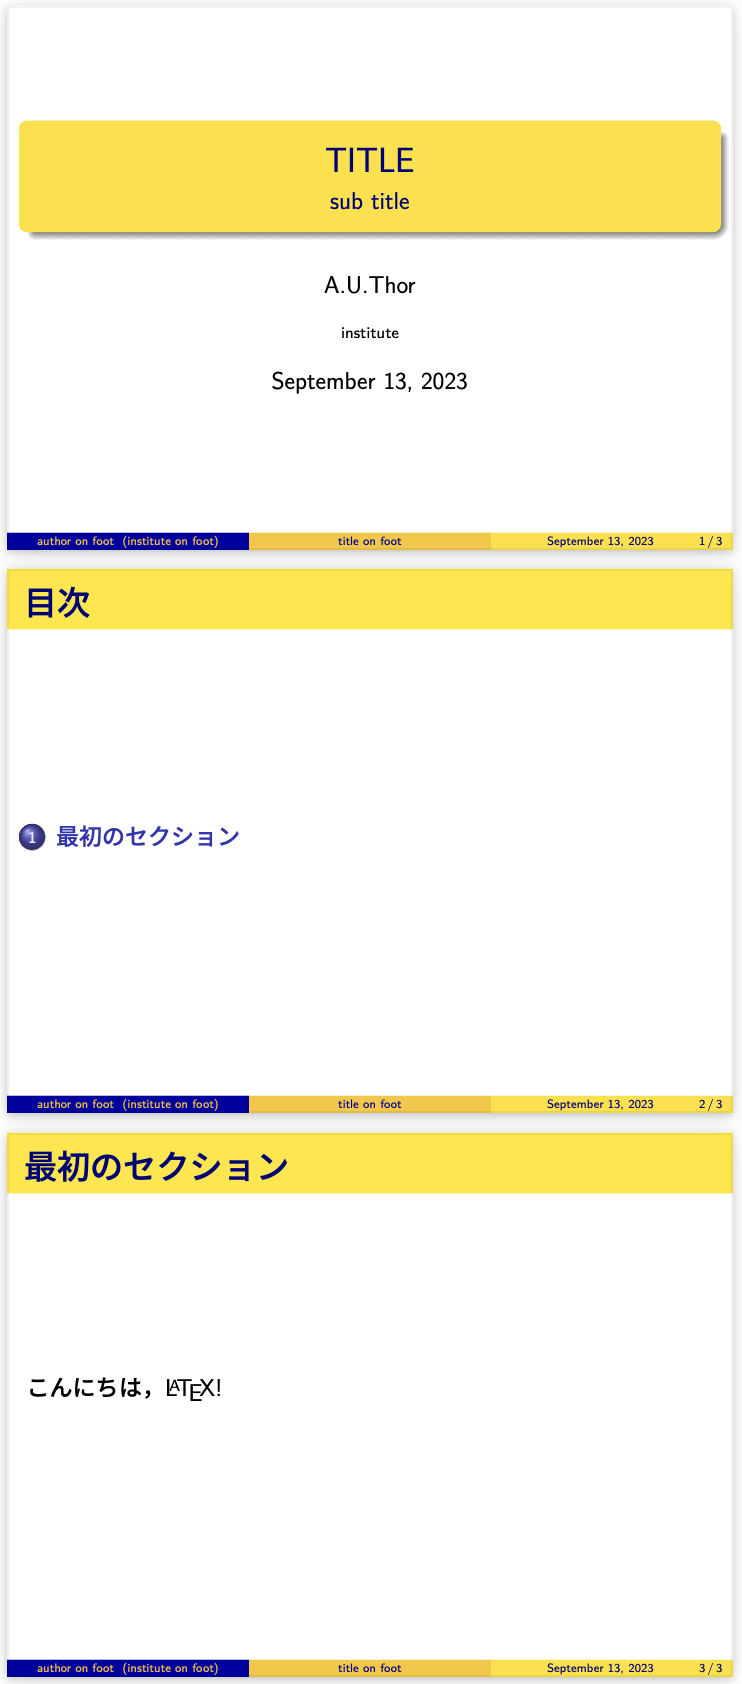
\includegraphics[width=\linewidth]{Madrid_wolverine.png}
  \end{textblock*}
\end{slides}

\begin{frame}[fragile]
  \frametitle{\secname\ (3/3)}

  \begin{itemize}
    \item \verb|theme|と\verb|color theme|を組み合わせればそれなりに色々なスライドが作れる \citep{beamer-gallery,beamer-theme-matrix}
    \item 自作のを公開している人も\citep{qiita-beamer-theme,ultimate-beamer-theme}
    \item \verb|\documentclass{beamer}|のオプションに
    \begin{itemize}
      \item \verb|[8-12,14,17, or 20pt]|で全体のフォントサイズ変更
      \item \verb|[aspectratio=43 or 169]|でアスペクト比変更
    \end{itemize}
    \item 自作するなら\verb|\setbeamerfont, \setbeamercolor,|\\
    \verb|\setbeamertemplate|とか
    \item 実は\verb|\note|コマンドで発表者用ノートも作れる
    \item 動画も頑張れは添付可(連番画像アニメーション)
  \end{itemize}
  



\end{frame}




\section[App B]{付録B}
\begin{frame}
  \frametitle{\secname}

  

\end{frame}

\end{document}